\chapter{Android Patterns Checks}

\section{Android Lint}

Android Lint é uma ferramenta oficial disponibilizada pela Google no Android 
Development Toolkit que analisa o código-fonte de projetos Android em busca de 
potenciais erros. Está disponível tanto como uma ferramenta de linha de comando, 
quanto integrado com IDEs, como o Android Studio. Exemplos de erros analisados incluem:

\begin{itemize}
  \item{Traduções incompletas (e traduções não utilizadas)}
  \item{Problemas de performance de layout}
  \item{Recursos (arquivos de imagens e sons, por exemplo) não-utilizados}
  \item{Problemas de internacionalização e acessibilidade}
  \item{Problemas relacionadas a ícones}
  \item{Problemas de usabilidades}
  \item{Erros no arquivo de manifesto}
\end{itemize}

Atualmente, o Android Lint possui cerca de 190 regras, que agrupam os erros em 
diversos graus de severidade e categorias. Os graus de severidade são 5, que vão 
de apenas informativos, onde não necessariamente é um erro mas que algo no código 
deve ser analisado, até fatal, em que existe um erro crítico no projeto, a ponto 
de falhar a criação do arquivo APK. Quanto às categorias podemos encontrar segurança, 
acessibilidade, internacionalização, usabilidade entre outras. Analisando essa 190 
regras previamente definidas, podemos relacionar cerca de 70 com algum tipo de 
variabilidade ou padrão definido pela plataforma. Como exemplo, podemos citar as 
regras "ButtonOrder", que verifica se a ordem dos botões na interface estão de 
acordo com o padrão de design sugerido pela documentação oficial e "NewApi", 
relacionado a variabilidade de versões da API, que aponta chamadas de métodos 
não-disponíveis em todas as versões da API para qual a aplicação foi desenvolvimento 
(de acordo com a versão mínima específica no arquivo de manifesto). O anexo X 
apresenta uma lista completa dessas regras. % TODO finalizar essa frase...

Para que o Android Lint aplique a analise de uma regra é necessário definir quais 
regras deverão ser utilizadas, o que pode ser feito no arquivo {\it build.gradle} do 
projeto na seção {\it lintoptions}, conforme mostra figura \ref{lintoptions}:

\begin{figure}[h]
    \centering
    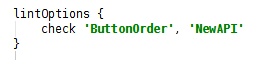
\includegraphics[width=5cm]{img/lintoptions}
    \caption[]{Trecho do arquivo build.gladle, indicando que as regras ButtonOrder e NewApi devem ser executadas}
    \label{lintoptions}
\end{figure}

